\chapter[Approach]{Approach}
\label{cap:Approach}
\begin{Resumen}

Within any industrial environment, a substantial and non-equivocate representation of the matter of study can be the most useful and time-saving tool, enabling performance boosting, yet as standardization. This chapter aims to illustrate the skill ramp-up performed so as to acquire and master the 2 main axes of the internship: i.e. \nameref{sec:approach:cim} and \nameref{sec:approach:software}, both required for convenient \nameref{sec:approach:project-approach} and contextualization.
\end{Resumen}
\PartialToc
\bigskip

\lettrine[lines=2]{\textbf{F}}{}rom the beginning of the \ingles{stage}, 2 principal axes were presented as main objectives of it, such as the \hyperref[sec:approach:cim]{Common Information Model (CIM)}, in addition to \hyperref[sec:approach:software]{all the sotware necessary} for its accomplishment: e.g. \nameref{sec:approach:software:matlab}, \nameref{sec:approach:software:FME} and the binomial  ESRI - \nameref{sec:approach:software:ArcGIS}.

\section{Introduction}
\label{sec:Diagram:intro}

These bidirectional objectives constituting a substantial skill rump-up, the first month and a half was basically framed on the familiarization with the tools and knowledge for such a purpose, and were aligning in the course of their learning. 

Indispensably, the author had to raise conscience of the problematic by gradually discretizing the problem and getting to get to know the departmental operation procedures, yet as the normative in the matter (specially regarding CIM schemes procedures). Once involved in the bureaucratic constraints implied, a theoretical introduction of the electrical devices seek to represent was stated.

Once the \ingles{Cahier des charges fonctionnel\footnote{Requirements specifications in french.}} stated, one was interested to the feasible technical solutions to sort it out. In the first instance, a \hyperref[sec:approach:software:matlab]{Matlab}-oriented approach was pursued, since the author felt much more comfortable with this tool. Those technical requirements going beyond the Matlab knowledge, project approach radically turned around, orienting towards the already used tools, and the departmental know-how, easing other members' skill transfer. 

Thereafter, the marked objectives visibility clarified notably, being two main axes the common thread of my project's contribution, from which certain structural sub-objectives could be identified:

\begin{itemize}
    \item \textbf{CIM}
    \begin{itemize}
        \item \textit{Familiarization:} 
        Becoming familiar with databases structuring and class arguments settlement is not easy and time-consuming.
        \item \textit{Standardization conscience-raise:}
        Standardizing any industrial application is a maximum if we want our project to remain accessible and functional in time and space.
        \item \textit{Normative constraints:} 
        Similarly, standardization objectives add difficulty to the problem, as they reduce its flexibility.
    \end{itemize}
    
    \item \textbf{Software deployment}
    \begin{itemize}
        \item\textit{Network model builder:} In charge oas seen inf databases-field assembling, by retaking class elements and re-affecting to those related in the fieldwork. Furthermore, hierarchical arboresecence confers the model its utility and veracity.
        \begin{itemize}
            \item FME: Powerfull Extract-Transform-Load (ETL) software for geographical, imagery and vectorial databases, used in data warehousing.
        \end{itemize}
        \item \textit{Displaying engine}
        \begin{itemize}
            \item ESRI: Being the world's most powerful mapping and analytics software, it furnishes with the best Geographic Information System (GIS) systems, such as ArcGIS or ArcMap. 
            \begin{itemize}
                \item \textit{ArcGIS} provides contextual tools for mapping and spatial reasoning and greater insights gaining by using contextual tools to visualize and analyze your data
            \end{itemize}
        \end{itemize}
    \end{itemize}
\end{itemize}

The sourcing quality of the virgin files used has deeply evolved along with the project. For that, an internal research was performed among the similar existing projects in Rte, successfully finding numerous adherence and certain exploitation possibilities. Thus, our original files, previously fed on completely chaotic and untidy RDF-formatted files, the exchanges with Stanway, then with Apogee have let us to base on much more relying and performant files. Whatsoever, files quality is still under study\footnote{An assessment study of Stanway's XML files' accuracy and rigurosity is currently being performed by ABB. Lille SRC's zone has already been validated, yet the rest of France remains under constant modifications.}, and  their evolution seems to be vital for the scrupulous representation of the entire France.

Once convinced of FME possibilities, a basic introduction to \nameref{sec:approach:cim} and \nameref{sec:approach:software:FME} conducted problematic awareness. Both FoS are quite technical and require lots of time for acquiring the technical competences at a professional level. The subsquent months supposed a continuous learning process and reciprocal contributions on more complexified matters (e.g. \nameref{sec:AIG:layout_optimization} techniques such as \nameref{subsub:AIG:SLV:graph_theory}, \nameref{subsub:AIG:SLV:MDS}, etc) from the individual to the project  and viceversa. These notions being implemented in \nameref{sec:approach:software:ArcGIS} toolset, and specially with \textit{Network Analyst}.

\begin{table}[h] \centering
\label{tab:margenes}
\caption{Month-to-month project time management procedure in weeks}
\begin{tabular}{lcc}
\toprule
\textbf{Project Time - Management template}  & & \\ \toprule
Phase description & Phase time(w) & Elapsed Time(w) \\ \midrule
Project dimension and finality acknowledgement & 1 & 1 \\
\textit{- First Matlab-driven post-level prototype} 	& 1.5 & 2.5\\
Reassessement & 1 & 3.5\\ \midrule
\textit{- Second Matlab-driven post-level prototype} & 1 & 4.5 \\
Software limitations awareness and reformulation &	2.5 & 7 \\ \midrule
FME skill ramp-up\footnote{This process has been markedly continuous and encompassed along the whole internship length.} &	2 & 9\\
\textit{- First FME Excel-driven zone-level prototype} & 1 & 10 \\
CIM corporate databases understanding &	1 & 11\\
\textit{- First FME CIM-driven zone-level prototype} & 2 & 13 \\ \midrule 
Standardization and Stanway know-how exchanges &	1 & 14 \\
\texttt{BusbarSection - Bay} notions - Modularization &	1 & 15\\
\textit{- Second FME CIM-driven zone-level prototype}& 0.5 & 15.5\\
\texttt{ACLineSegment} interposts notion introduction  & 0.25 & 15.75\\
Crossing-edges solution + ArcGIS interface dumping &	1.25 & 17\\ \midrule
\textit{- First ArcGIS zone-level prototype}&	0.5 & 17.5\\
Graph theory and layout management skills ramp-up & 1.5 & 19\\ 
FME position management import - looping &	1.75 & 20.75\\ \midrule
ArcGIS toolset (\textit{Network Analyst}) conscience raisement &	0.75 & 21.5\\ 
\textit{- First ArcGIS prototype} & 2.5 & 24\\ \midrule
Industrialization - Normative and reports writing & 2 & 26 \\
\midrule
\textbf{Total project time}& \textbf{26} &\textbf{26} \\
\bottomrule 
\end{tabular}
\end{table}

Time expended on each of these phases is specified in \href{the table hereafter}{tab:margenes}, for the reader to form a complete idea of how the pro jet evolved through project progress and personal skill ramp:

\begin{figure}[h]
    \centering
    \parbox[t]{1\textwidth}{
    \href{}{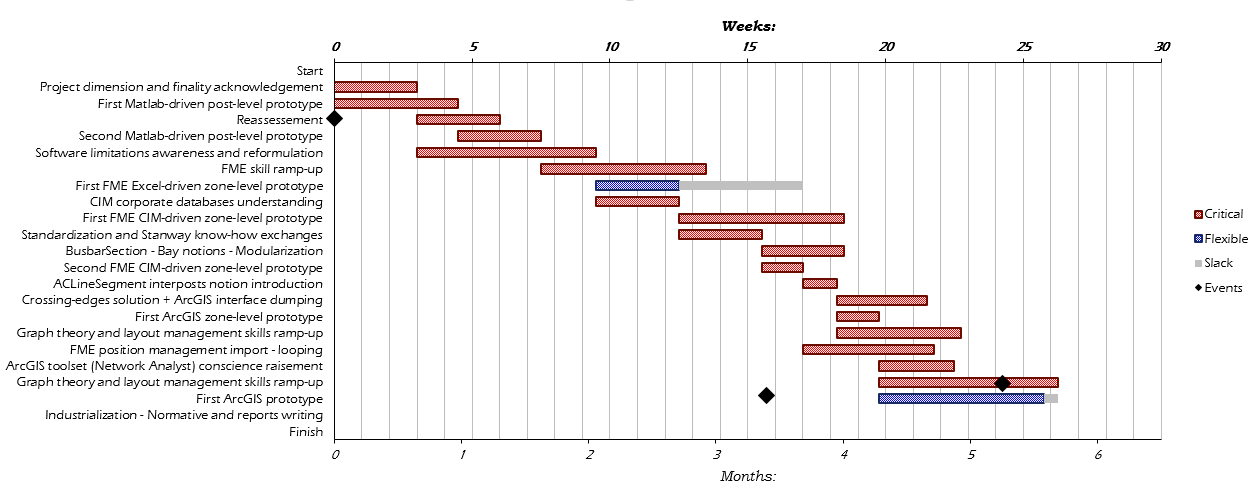
\includegraphics[width=1\textwidth]{0.figuras/Gantt-proejct.png}}
    \captionof{figure}{Gantt project management chart.}
    \label{fig:Gantt-diagram}}
\end{figure}

As in any project, its management seemed vital ff or resources optimizing and incertitude confronting. To this effect, a \hyperref[fig:Gantt-diagram]{Pert-Gantt chart binomial diagram} has been made in the incertitude phases of the project, assessing its control and tackling all the project long equally. To this effect, critical path and important tasks were identified constraining therefore their duration, yet as their potential impact in the whole project duration.

% ---------------------------------------------------------------------

\section{CIM}
\label{sec:approach:cim}

In electrical power industry, CIM refers to the standard developed by the International Electrotechnical Commission (IEC) and industrialized by Electric Power Research Institute (EPRI), with the support of the North American Electric Reliability Council (NERC), striving to normalize electrical network information exchanges between software applications\cite{IEC_CIM_static}. UML modeled IT environment, elements are represented as classes and any relationships between them are considered as associations. Inheritance allows specialization of common base elements into more specific derived elements.

From the perspective of Geographical Information Systems (GIS) users, CIM provides a useful data exchange schema for electrical objects \cite{CIMIntelliGrid}, and is of primary importance for layout support and communication with other applications. In addition, the paradigm shift around principal leading enterprises towards GIS network harvesting technologies enables CIM modeling harnessing for automatically reconstruct network diagram layout \cite{CIM-GIS}.

\subsection{Normative}

Through normalizing regulatory international framework, and in pursuit of databases standarization, application software integration is eased,  regarding any kind of energy transmission (explicited in \texttt{IEC 61970-301} \cite{IEC-2003}) and market communications (\texttt{IEC 62325}), normally portrait in  XML or RDF formats (\texttt{IEC 61970-501} \cite{IEC_xml-rdf} and \texttt{61970-452} \cite{IEC_CIM_static}).  

Ultimately, it is notably \texttt{IEC 61968} \cite{IEC-application} series of standards, plus the IEEE delivrables \cite{CIMIEE,CIMIntelliGrid} who extend CIM possibilities to meet the needs of electrical distribution in terms of distribution, work and outage management systems, planning, metering, geographic information system, asset management, customer information systems and enterprise resource planning. 

\subsection{Concept, utility and key aspects of CIM}

\textit{"An information model is a representation of concepts, relationships, constraints, rules, and operations to specify data semantics for a chosen domain of discourse"} (Y. Tina Lee, Information Modeling: From Design to Implementation, NIST, 1999): such an abstract definition enunciated 20 years ago remains completely valid on these days and perfectly depicts the proof of concept and interest of CIM, and of any Model Dreiven Architectures (MDA) logic generically. 

At that time, the need of a rigorous, logical yet versatile platform became increasingly apparent for massive data quantities management, notably on object regrouping and indexing, for better performance achievements, giving birth to multiple key dimensions that widespread in the recent years. Big Data, Intelligent behaviour or Internet of Things concepts are based on this concept.

Returning to the subject of CDL automatizing, by abstracting CIM knowledges, and applying them to the patrimonial databases, a double-sense impact on our study was obtanied: First it will contribute to the standarization of the patrimonial databases \cite{cahier_dpc2,guide_GAI,Note_accompagenement}, and secondly, it will decomplexifiy the problem, by clarifying the electrical elements to represent idiomatic structures. In our case, electrical elements were identified in different classes, as defined in \nameref{Acronyms} chapter. Each of them responding to a element on field and the most important being:

\begin{multicols}{3}
\begin{itemize}
\item \textit{ACLineSegment
\item BaseVoltage
\item Bay
\item Breaker
\item BusbarSection
\item ConnectivityNode
\item ConductingEquipement
\item Disconnector
\item EnergyConsumer
\item GeneratingUnit
\item Line 
\item LinearShuntCompensator
\item LoadBreakSwitch
\item PowerTransformer
\item PowerTransformerEnd
\item SynchronousMachine
\item Terminal
\item VoltageLevel}

\end{itemize}
\end{multicols}


Files initially used were RDF-structured, with linking chain attributes given in alphanumeric as those appearing in \hyperref[fig:RDFformat]{the following image}, where even though the introduction of a primer hierarchical notion was presented, one could nonetheless confer how absolutely no elements sorting and poor attributes enrichment was performed:


\begin{figure}[h]
    \centering
    \parbox[t]{0.6\textwidth}{
    \href{}{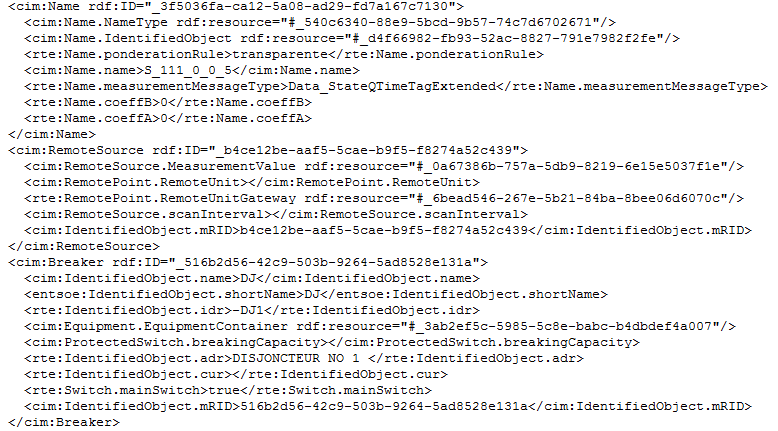
\includegraphics[width=0.6\textwidth]{0.figuras/RDF_database_format.png}}
    \captionof{figure}{Original RDF files appearance. A fragment from \texttt{GDP-AMIENS.rdf} displayed.}
    \label{fig:RDFformat}}
\end{figure}

This fact  notably contributing to data treatment engrossment and even often provoking data losses and rigorousness faibleness, a change to \hyperref[fig:XMLformat]{XML files} notably improved their clarity and structuring. Anyhow, the main hierarchical core of the treatment was maintained, whereas data quality fortly pare its complexity down. 

Thenafter, network elements were subsequently organized in different classes and characterized by their attributes in a ordered and logical way. Those classes being continent and content of others spawn an arborescent and structurally logical model, the metadata structure is transparent and bijective with regards to on-field architecture hierarchy.

\begin{figure}[h!]
    \centering
    \parbox[t]{0.8\textwidth}{
    \href{}{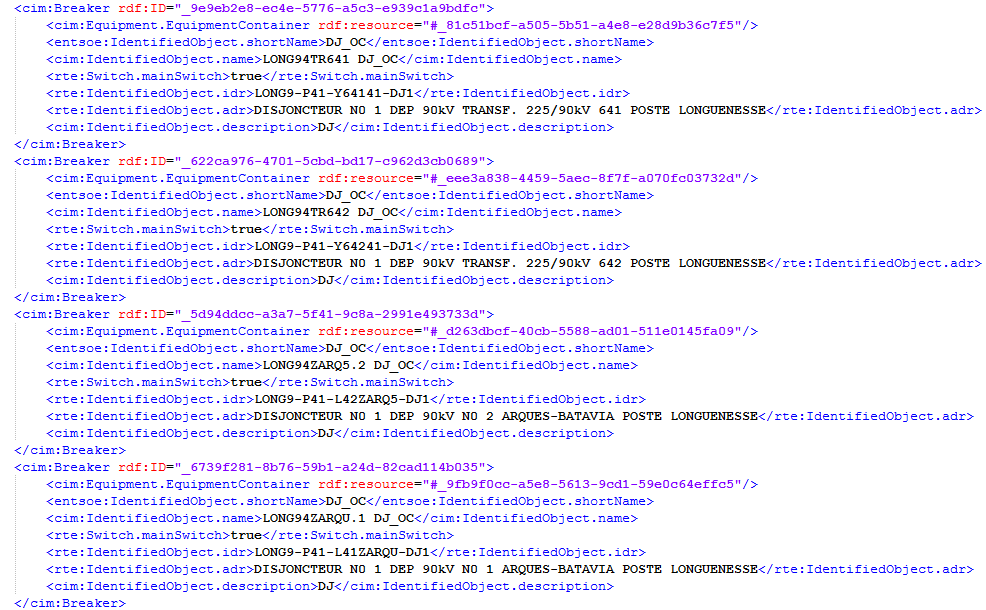
\includegraphics[width=0.8\textwidth]{0.figuras/XML_database_format.png}}
    \captionof{figure}{Stanway XML files appearance. Here, \textit{Breaker} class, from \texttt{V1-00-40-LILLE.xml} file is displayed.}
    \label{fig:XMLformat}}
\end{figure}

As it will be shown in deep all along \nameref{cap:AIG} chapter and particularly in \autoref{tab:classes_XML} is pretty well-illustrated, priorizing the classes as well as identifying relevant attributes to join all them is prior to understand and extend the UML model as it was conceived by the designer\cite{CIMIntelliGrid}. Those attributes (\textit{ACLine Segment, BusbarSection, Breaker, GeneratingUnit}) normally take unequivocally and hierarchically account of in-field switch-gear(which  will refer to an Intersubstatinons connection line, a Busbar, a Position breaker or a Power Generator reciprocally). Indeed, \autoref{fig:CIM_diagram-layout} enables to easily identify how the different topological structures contained in a 3-positions post, each of them pointing toward a different voltage level is non equivocally correlated to a different \textit{VoltageLevel}\footnote{Referring to the broken-line square regrouping the different tension levels (and not the \textit{PowerTransformer} nor the \textit{ACLineSegment} for example).}.

Attributes assembling and arranging, as deeply exploited in \nameref{subsubsec:AIG:methodology:structurisation:topology} sub-chapter, enabled discernive representation in \nameref{sec:approach:software:ArcGIS} through layers regrouping and intelligent displaying\footnote{Standards indicate than rates of 1000 objects-per-screen are adequate for a good discerning displaying.} optimization.

\subsection{Diagram layout}
\label{sec:approach:diagram_layout}

The ability to visualize network schematics can be critical for engineers when interpreting the status of an electrical network. As the number of interlocutors utilizing electrical models grows and utilities move towards a common network model across applications, the drive to ensure \hyperref[sec:approach:diagram_layout/SLD]{single line diagrams} are accurately reproduced in a standard and performant way sharpens progressively.

CDL format extends CIM to provide a mechanism for standardizing how the layout of electrical schematics is displayed, relaxing  graphics and network data exchange, while ensuring that schematic views are synchronized with the electrical model across multiple systems, such as \nameref{sec:approach:project-approach:parties:stanway}'s or \nameref{sec:approach:project-approach:parties:apogee}'s, regarding our corporate framework. In other words, this standard is intended to allow each of those system to accurately recreate the layout sought, by using their own styling for icons, colors, fonts and other graphical rendering attributes, while keeping their exceptional functionalities on the margins. 

\begin{figure}[h!]
    \centering
    \parbox[t]{0.7\textwidth}{
    \href{}{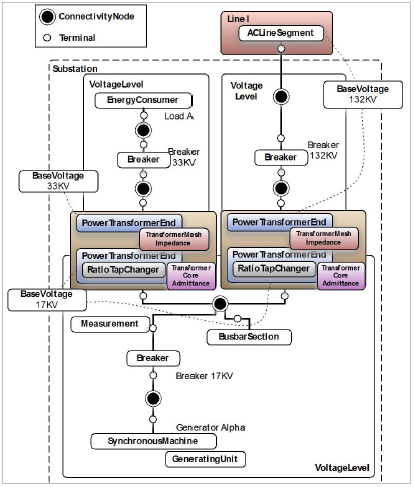
\includegraphics[width=0.7\textwidth]{0.figuras/example_CIM_mapping_UML-structure.png}}
    \captionof{figure}{CIM structural data skeleton and classes interdependances. Example Circuit with Partial CIM Class adjacences \cite{CIMIntelliGrid}.}
    \label{fig:CIM_diagram-layout-skeleton}}
\end{figure}

This way, elements can be systematically represented in common and standartized criterial specifications and, if sourced on the same patrimonial databases\footnote{as it is actually intending between Stanway's and Herge's at the momment.}, architectural structure of the represenation will be completely transposable, regardless of the particularities of each functional tool. To illustrate this fact, backtracking on the post representation subject, this structure could be extended and parametrised in such a way that the final representation of a certain post (retaken s seen in \autoref{fig:CIM_diagram-layout-skeleton} logic) will be the same and completely evident to the actual display, notably that of\hyperref[fig:CIM_diagram-layout]{the figure here below}.

On this pursuit, \textit{Terminal} and \textit{ConnectivityNode} notions are extremely important as they are in charge of the subsequent elements linking, specially when several attached to a similar post, as displayed in \autoref{fig:post_XML_structure-Terminal} in the following. Electrical network standards criteria has been respected in object representation, where different constraints have been established in pursuit of diagram layout adapting to the requirements specified in \cite{CIMIntelliGrid}.

\subsubsection{Single-line high voltage electric diagrams}
\label{sec:approach:diagram_layout:SLD}

Reducing the three-phase power system representation of the evoked example to SLD standards, the final appearance of the aggregated classes automatic and properly-ordered layout display would be as follows:

\begin{figure}[h!]
    \centering
    \parbox[t]{0.7\textwidth}{
    \href{}{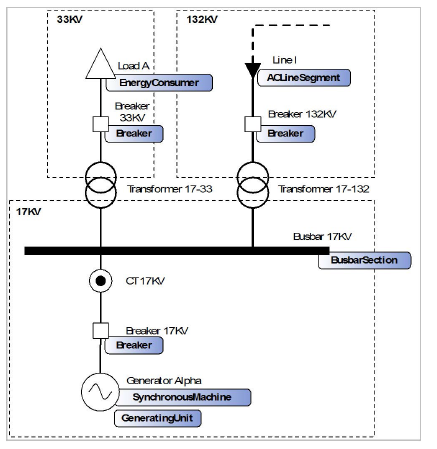
\includegraphics[width=0.7\textwidth]{0.figuras/example_CIM_mapping.png}}
    \captionof{figure}{CIM structure projection on diagram layout representation. Example Circuit with Partial CIM Class Mappings \cite{CIMIntelliGrid}.}
    \label{fig:CIM_diagram-layout}}
\end{figure}

Such a tedious task was traditionally performed by teams of architects who manually drew the complete SRC and SNC schematics in AutoCAD. In this, no optimization criteria was stated apart from the personal experience of the designer, which obviously, remained purely subjective. To this extent, several assessment criteria have been established in the wake of several meetings convened with \hyperref[sec:approach:project-approach:parties]{the different concerned parties} to identify common interests, as well as eventual divergences inter projects, and thus fix a common criteria consequentially. 

At any rate, all the stakeholders agreed that any automatizing could not be performed in a coherent extend unless international procedures regarding CIM database settlement and exploitation legislature \cite{CIMIntelliGrid, CIMIEE}, plus those existing on electrotechnical representation of HV schemes were totally respected individually and threaded together.

\subsubsection{Spread-out of technology impact on diagram representation}


is driving progress on this  integrated approach across
Several software applications have been traditionally used for functional design, physical design, and asset tracking, being \textit{Actrix Technical 2000}, from \textit{Autodesk}, and \textit{Visio 2000 Technical Edition}, from \textit{Microsoft} the most widely known. Nonetheless, few affordable software applications integrate all of these capabilities combining an interactive graphical interface with links to pertinent data for a comprehensive, yet easy-to-learn-and-use technical drawing environment.

That is the reason why numerous enterprises have been recently seduced by the idea of automatizing their corporate schemes through patrimonial databases plus Application Program Interface (API) tools exploitation. ORACLE,  JavaScript\cite{automatic-orthogonal-graph,CIMjava}, GIS programs... the demand on highly-skilled employees on the matter is definitely and remarkably growing, so does the identification of those needs. 

In addition, numerous technologies could benefit from the development of this, for the moment, merely-scientific-techniques on an industrialized approach, due to its transponability possibilities: \textit{Pajek} and \textit{Tulip} for big networks visualization \cite{aig-state-of-art-softwares} are the mainstream tools. Diagrams visualization can be performed static (\textit{Graphviz} (in multiple formats)) and dynamically (\textit{Dynagraph}), along with \textit{yFiles} for archives formatting, \textit{DBdraw} for Relational Databases or \textit{Govisual} for UML Class Diagrams, being most of this technologies developed in Eclipse Modelling Framework (EMF) platform.

Development of this software toolset is driving progress on this integrated approach across Business Process Model and Notation (BPMN) automatic layout \cite{automatic-layout-bpmn}, Assets adjustments on Mental Mapping \cite{layout-adjustement-mental-map}, automatic orthogonalistaion of graphs \cite{automatic-orthogonal-graph} or automatic similarity relationship assessment in bioinformatics \cite{algorithm-biological-data}.

ACERCAR LOS EJEMPLOS ALGO MAS A LO QUE HAGO YO => MEJORAR LA BUSQUEDA Y CAMBIAR LAS CITAS.

\section{Software deployment}
\label{sec:approach:software}

Acknowledging which tool meets our needs best comports a non-negligible marginal weight of the whole project success, yet it could even risk losing its route if a previous state-of-art effort is not undertaken. In my case, this stage took several time, as multiples possibilities in terms of software deployment seemed to be feasible, notwithstanding forget that my technical skills on the use of most of them chosen were more than poor at the beginning of the internship.

Thus, by shifting from an only Matlab interface prototype \nameref{sec:approach:software:matlab} to the final implementation of an intelligent, adaptable and performing representation system by using \nameref{sec:approach:software:FME} for the architectural part, and \nameref{sec:approach:software:ArcGIS} for the purpose of displaying optimization, the possibilities and perspectives of the project approached evolved considerably. Through all this software use, modularity has been a maximum prioritizing latters work restart and whole project industrialization.


Inter alia, those 2 software are mainly preponderant on the setting up of Herge's diagram layout automatizing, so are the stages in which this layout has been reached. In so doing, a first stage of data treatment and analyzing has been performed in \nameref{sec:approach:software:FME}, comprising this part the major part of the time passed. Secondly, a post-data treatment process resulting from \nameref{sec:approach:software:ArcGIS} activities took place, much less time consuming and evident, where post positions and even breakers' was modified so as to optimize the whole representation. Positions which were initially given by files extracted from DPC\textsuperscript{2}, and experimented several transformations thanks to the\nameref{subsub:AIG:SLV:graph_theory:meta_algorithms} implemented in \nameref{sec:approach:software:ArcGIS}. 

As recurrently cited, different files formatting were used all over the project, which was possible to the flexibilization of the entry-exit flux of data. This versatility was possible thanks to \hyperref[fig:FMEversatility]{FME's understanding capacity of the different formats imported}, and there sustains the  criteria decision of its choice. COMPLETAR

\subsection{Matlab}
\label{sec:approach:software:matlab}

In a first approach, the user felt much more confident on using Matlab for digital projection of the existing architecture on-field. Therefore was it chosen for a primal project requirements approach, enabling a conscience-raising in addition to a know-how corporate ramp-up. At any case, we must distinguish that the idea that Matlab was evidently not the proper software for the final implementation for the service was always acknowledged, although user was not yet technically aware enough for its correct implementation. 

The approach undertaken consisted on the creation of different post pictograph typologies through the use of several matrices disposition. This enforced technical knowledge on electrical devices semantics and their schematics while introducing the corporate post typologies gradually. Therefore post location and bar positions were reproduced, with a posterior patch that enabled their coupling.

\begin{figure}[h!]
    \bigskip
    \begin{center}
        \parbox[t]{.475\textwidth} {%
        \href{}
            {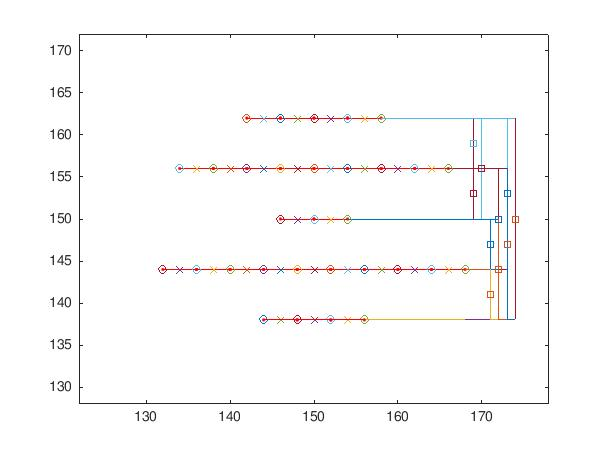
\includegraphics[width=.475\textwidth]{0.figuras/Matlab_postes_barres_generation.jpg}}}\hfill
        \parbox[t]{.475\textwidth}{\caption{Initial Matlab-oriented approach of a 5-barres-post design (all barres coupled).}
            \label{fig:matlab_design}}
    \end{center}
\end{figure}

Code is available on the \nameref{subsec:Appendix:Diagram:Matlab:code} subsection of Appendix. Its size and approach give full account of the limitations this canvass implied and so of the necessity of a more intelligent evolving perspective in term of software usage. 


\subsection{FME}
\label{sec:approach:software:FME}
That is, after a first Matlab-oriented approach (see \autoref{fig:matlab_design}), the author could thus raise conscience of the project dimension, and so that, of the necessity of a much more data-oriented software.

The major bulk of the work was performed using FME, began the moment the author introduced it on its data processing treatment, that is, at the beginning of the second month of the internship. With the worldwide mot used Spatial ETL application, the main part of the value-adding process aroused: thereafter, a new dimensional "thick-pipe"\footnote{Traditionally the software used to translate geographic data to a different format had limited capabilities. Most of the data would be forced through a limited data model causing much of the meaning to be lost in translation. We call this a “thin-pipe translation”.} translation method between databases integration on representation software became a reality.  

Spatial ETL tools can read, write, and manipulate spatial data (or not necessarily) in a whole array of supported semantic formats bijectively, streamlining data translation from one spatial database or GIS, CAD or raster graphics software to another. Those features were deeply exploited for posts representation in different coordinated systems inputting.

\begin{figure}[h!]
    \centering
    \parbox[t]{0.6\textwidth}{
    \href{https://www.safe.com/how-it-works/}{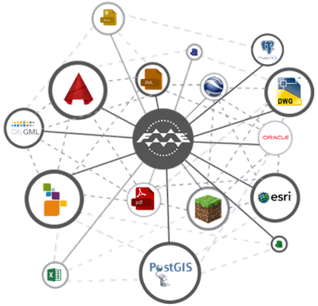
\includegraphics[width=0.6\textwidth]{0.figuras/FME_versatility.png}}
    \captionof{figure}{FME versatility leads to multiple format understanding possibilities}
    \label{fig:FMEversatility}}
\end{figure}

Plus, it offers a much more efficient and economic representation in terms of memory usage consumption, which, in view of the size of the files managed, implied a considerable computation power releasing of the processors corporative unit.
Furthermore, FME provides incredible performances in data consolidation and clarification, which strenghtened considerably blanks or incoherences presented on the imported XML files. Also, its online or and cloud working capabilities enabled multiples team working on a same file symustaniously and, what is more important, non concomitantly\footnote{In the futrure, \href{https://git-scm.com/}{Git}-formatted industrialization of the problem could enable multiple features introduction, such as versions controls or multiple users work enrichment.}. 

Outbound information form each treatment block is consecutively used and stocked in form of a blockchain\footnote{A block chain is a continuously growing list of records, called blocks, which are linked. Each block typically contains a cryptographic hash of the previous block, a timestamp, and transaction data.} tree, in which every block enriches the information contained in the chain. Those blocks being previously configurated and coded, make the class interusage activity much more intuitive. 

Given the high computational power needed, programs were run through a virtual machine (VM), whose IP, and therefore, whose server was shared among all the team members\footnote{Whatsoever, the team owned several VMs for different programs installation and launchment.}.

 
\subsection{ArcGIS}
\label{sec:approach:software:ArcGIS}

Currently, lots of controversy has been awaken since private geodata leaks are a never-end problem on the matter. Indeed, lots of software are capable of not only have access to our geographical position information, but also recross, parametrize or reassess it with others for assessing intelligent models of human behaviour, shortest-path opening business headquarters setting or automatic objects positioning for space optimization. \href{https://www.esri.com/en-us/arcgis/about-arcgis/overview}{ArcGIS, powered by ESRI} is the software used for pictographical projection of the previously FME-shaped network. By means of it, different infographies and images can be linked to FME objects class's typology, ensuring regulatory compliance. 
KEEP THE IMAGE??

\begin{figure}[h!]
    \centering
    \parbox[t]{0.8\textwidth}{
    \href{https://www.diatomenterprises.com/visual-data-representation-in-google-maps-bing-maps-or-esri-which-to-choose/}{
\includegraphics[width=0.8\textwidth]{0.figuras/googlemaps_bingmaps_esri.jpg}}
    \captionof{figure}{Representation systems are well spread among non-professional users. Google, Bing and other search engine have been including them on their mapping devices for some time now.}
    \label{fig:Googlemaps}}
\end{figure}

Geographical information coming from FME treatments was traditionally visualized with the integrated FME Data Inspector. Nevertheless, ArcGIS offers a much more efficient and economic representation in terms of memory usage consumption\footnote{In view of the size of the files managed, implied a considerable computation power releasing of the processors corporate unit}.

In addition, it enabled working with objects repositioning and their geographic information emerged, while improving displaying quality thanks to ArcReader performances. In particular, a vast range of enriched functionalities were systematically added to the process, chipping in the final result with some additional features. Thereby, several greater insights were gained by using contextual tools such as object layering thanks to ArcView and ArcEditor, which contributed to clarify the representation, while discretizing the object types, plus their adjacent information (ArcInfo) that was intended to be displayed, as well as it.

But what contributed the most to the problematic of study were ArcGIS spatial analytics features, which lead to spotting in the lattice network spatial patterns for more convenient redispositions, in the purpose of a certain objective funciton optimization. This algorithm, inspired in \nameref{subsub:AIG:SLV:graph_theory} principles, could be equally implemented in the future through on-field modifications with no-contribution  required (appart the patrimonial databases enrichement), as its setting up has been completely automatized.

ANADIR IMAGEN DE NETWORK ANALYST??

Real-time GIS empowers location monitoring for SCADA schemes, accelerating response times, optimizing safety, and improving operational awareness across all assets and activities, whether in motion or at rest. Moreover, data collection and management has been integrated in the corporate systems efficiently and securely.

Conversely, several issues were faced when geodatabase dumping between FME and ArcMap. This was due to the attributes formatting in the extracted document, which didn't always come from the same origin, so that their architecture and typology was neither. This ended up resulting on a non-canonical and unique data structuring. 

% ---------------------------------------------------------------------




